\documentclass[10pt]{article}
\usepackage{icmlko}

\icmlmeta{IP 파운데이션 월드모델}{159}{공휴일 하나, 그리고 크기를 안 보던 잣대}{달력 여섯 중 어느 것이 일하는지 찾았더니 공휴일 간격 하나였고, 그것이 고치는 축을 들여다보니 내 잣대가 크기를 안 세고 있었다}

\begin{document}

\twocolumn[
\icmlheader

\begin{abstract}
노트 158이 ``달력 여섯이 손 축의 개입 부호를 고친다''를 보이고 ``여섯 중
어느 것인가''를 남겼다. 하나씩 더해 봤다. \textbf{공휴일 간격 하나다.}
손 축 다섯만일 때 F18 배깅 72\% · F6 능형 58\%인데, 요일 사인 · 코사인 ·
주말 · 월 사인 · 코사인을 하나씩 더해도 58$\sim$75\%로 거의 안 움직이고
\texttt{cal\_holiday\_gap} 하나를 더하면 \textbf{81\% · 78\%} --- 달력
여섯을 다 넣은 것과 똑같다. 그것이 어느 손 축을 고치는지도 찾았다.
\textbf{장소 노출이다} --- F6 능형에서 개입 부호가 \textbf{0/7 에서 7/7 로}
뒤집힌다. 일곱 도메인 전부에서 음수이던 것이 전부 양수가 된다. 여기서
멈추지 않고 크기를 봤다. \textbf{$-$0.0061 $\sim$ $-$0.0021 이 $+$0.0016
$\sim$ $+$0.0044 로 바뀐 것이었다} --- 다른 축의 보통 크기가 0.039 이니
\textbf{10분의 1도 안 되는 양이 부호를 넘나든 것}이다. 방향은 체계적이지만
(일곱 도메인이 다 같이 움직인다) 양은 거의 없다. \textbf{그러니 내 잣대가
틀렸다} --- 단순 부호 일치율은 0.002짜리 칸과 0.06짜리 칸을 같은 무게로
센다. 크기로 가중해 다시 재니 그림이 달라진다. 손 축만으로도 F18 89\% ·
F6 \textbf{82\%}이고(단순으로는 58\%였다), 공휴일을 넣으면 92\% · 85\%다.
\textbf{달력의 기여가 $+$20\%p 에서 $+$3\%p 로 줄어든다.} 노트 158의
``달력이 부호를 지킨다''는 방향은 맞지만 크기는 6분의 1이었다. 그리고
크기 가중으로 보면 \textbf{축을 더 넣을수록 조금씩 좋아진다}(전부 19축이
93\% · 86\%로 최고) --- 노트 157이 세우고 노트 158이 반증했다고 적은 그
예측이 \emph{제대로 된 잣대에서는} 약하게 살아난다. \texttt{lab/lever.py}
로 묶어 실행마다 기록한다.
\end{abstract}
]

\begin{figure*}[t]
\centering
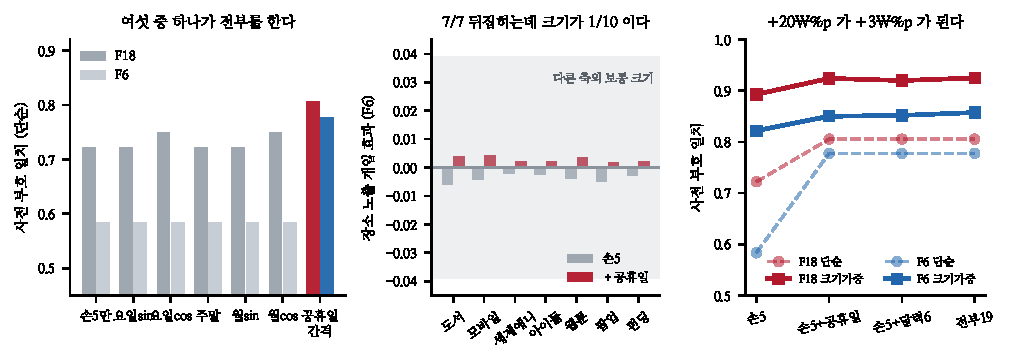
\includegraphics[width=\textwidth]{figs/holi.pdf}
\caption{왼쪽 --- 여섯 중 하나가 전부를 한다. 가운데 --- 7/7 뒤집히는데
크기가 10분의 1이다. 오른쪽 --- 잣대를 고치면 $+$20\%p 가 $+$3\%p 가 된다.}
\end{figure*}

\section{공휴일 간격 하나}

\begin{table}[t]
\centering\tsize
\caption{손 축 다섯에 달력 하나씩 더할 때. 사전 부호 일치(단순).}
\begin{tabular}{lrr}
\toprule
& F18 배깅 & F6 능형 \\
\midrule
손5만 & 72\% & 58\% \\
$+$ 요일 사인 & 72\% & 58\% \\
$+$ 요일 코사인 & 75\% & 58\% \\
$+$ 주말 & 72\% & 58\% \\
$+$ 월 사인 & 72\% & 58\% \\
$+$ 월 코사인 & 75\% & 58\% \\
\textbf{$+$ 공휴일 간격} & \textbf{81\%} & \textbf{78\%} \\
\midrule
($+$ 달력 여섯 전부) & 81\% & 78\% \\
\bottomrule
\end{tabular}
\end{table}

\claimx{\textbf{공휴일 간격 하나가 달력 여섯과 똑같다.} 나머지 다섯은
합쳐도 F6 에서 한 칸도 못 고친다.}{말이 된다 --- 팝업은 연휴에 맞춰
잡히고 연휴 근접이 방문객을 움직인다. 요일과 월은 그보다 거친 대리이고,
이미 공휴일 간격이 담고 있다.}

\section{고치는 축은 장소 노출이다}

\begin{table}[t]
\centering\tsize
\caption{손 축별 사전 부호 일치. 맞은 도메인/전체.}
\begin{tabular}{lrrrr}
\toprule
& \multicolumn{2}{c}{F18} & \multicolumn{2}{c}{F6} \\
& 손5 & $+$공휴일 & 손5 & $+$공휴일 \\
\midrule
타깃 폭 & 9/9 & 9/9 & 9/9 & 9/9 \\
미디어 푸시 & 4/4 & 4/4 & 4/4 & 4/4 \\
굿즈 규모 & 7/8 & 8/8 & 8/8 & 8/8 \\
\textbf{장소 노출} & 4/7 & 5/7 & \textbf{0/7} & \textbf{7/7} \\
입장 마찰 & 2/8 & 3/8 & 0/8 & 0/8 \\
\bottomrule
\end{tabular}
\end{table}

\claimx{\textbf{능형에서 장소 노출이 0/7 에서 7/7 로 통째로 뒤집힌다.}
F6 의 58\% $\to$ 78\% 는 거의 전부 이 축 하나다(일곱 칸).}{연휴에 좋은
자리가 배정된다 --- 1층 아트리움 · 정면 매대는 성수기 물건이다. 공휴일을
안 넣으면 장소 노출이 그 몫을 대신 진다.}

\section{그런데 크기를 봤다}

\begin{table}[t]
\centering\tsize
\caption{F6 · 장소 노출의 도메인별 개입 효과.}
\begin{tabular}{lrr}
\toprule
& 손5 & $+$공휴일 \\
\midrule
도서 & $-$.0061 & $+$.0038 \\
모바일 & $-$.0044 & $+$.0044 \\
웹툰 & $-$.0039 & $+$.0036 \\
팝업 & $-$.0050 & $+$.0016 \\
펀딩 & $-$.0026 & $+$.0022 \\
아이돌 & $-$.0026 & $+$.0022 \\
세계애니 & $-$.0021 & $+$.0023 \\
\midrule
\textbf{평균 $|\cdot|$} & \textbf{.0038} & \textbf{.0029} \\
(다른 축의 보통 크기) & \multicolumn{2}{r}{\textbf{.039}} \\
\bottomrule
\end{tabular}
\end{table}

\claimx{\textbf{10분의 1도 안 되는 양이 부호를 넘나든 것이다.} 일곱 칸이
전부 뒤집혔지만 움직인 폭은 0.002$\sim$0.006이고 다른 축의 보통 크기는
0.039다. 능형은 장소 노출을 어느 쪽으로도 거의 안 쓴다.}{방향은 잡음이
아니다 --- 일곱 도메인이 다 같은 쪽으로 움직였다. 무작위 부호라면
$2^{-7}$ 이다. \textbf{체계적이지만 미미하다}는 것이 정확한 서술이다.}

\section{그래서 잣대를 고쳤다}

\claimx{\textbf{단순 부호 일치율은 0.002짜리 칸과 0.06짜리 칸을 같은 무게로
센다.} 그래서 F6 능형이 58\%로 보였는데, 크기로 가중하면 \textbf{82\%}다.
틀린 칸이 전부 작은 칸이었다.}{노트 155 · 156 · 157 · 158이 이 잣대를 썼다.
방향은 다 살아남지만 크기는 다시 읽어야 한다.}

\begin{table}[t]
\centering\tsize
\caption{잣대를 고치면.}
\begin{tabular}{lrrrr}
\toprule
& \multicolumn{2}{c}{F18} & \multicolumn{2}{c}{F6} \\
& 단순 & \textbf{가중} & 단순 & \textbf{가중} \\
\midrule
손5 & 72\% & \textbf{89\%} & 58\% & \textbf{82\%} \\
손5$+$공휴일 & 81\% & \textbf{92\%} & 78\% & \textbf{85\%} \\
손5$+$달력6 & 81\% & 92\% & 78\% & 85\% \\
\textbf{전부 19} & 81\% & \textbf{93\%} & 78\% & \textbf{86\%} \\
\bottomrule
\end{tabular}
\end{table}

\claimx{\textbf{달력의 기여가 $+$20\%p 에서 $+$3\%p 로 줄어든다.} 노트 158의
``달력이 부호를 지킨다''는 방향은 맞지만 크기가 6분의 1이었다.}{그래도
$+$3\%p 는 검색 축의 $+$0\%p 보다 크고, 판 $\rho$ 를 $-$0.038 깎으면서
얻는 것이라 노트 158의 ``통제''라는 읽기 자체는 유지된다.}

\claimx{\textbf{그리고 노트 157의 예측이 약하게 살아난다.} 크기 가중으로
보면 축이 늘수록 조금씩 좋아진다 --- 89 $\to$ 92 $\to$ 93(F18), 82 $\to$
85 $\to$ 86(F6). 노트 158이 ``반증됐다''고 적은 것은 \emph{단순} 잣대에서
그랬던 것이다.}{$+$1\%p 씩이라 여전히 약하다. ``더 넣으면 좋아진다''보다는
``더 넣어도 안 나빠진다''가 정확하다.}

\section{묶었다}

\texttt{lab/lever.py} 로 묶고 \texttt{lab/loop.py} 의 실행 요약에
\texttt{lever\_plain} · \texttt{lever\_weighted} · \texttt{lever\_size} 를
싣는다. 노트 144의 귀착, 노트 146의 씨앗, 노트 147의 짝 분해능에 이어
넷째 부기다.

\begin{table}[t]
\centering\tsize
\caption{남은 것.}
\begin{tabular}{ll}
\toprule
입장 마찰 & F6 에서 0/8 --- 공휴일로도 안 고쳐진다 \\
크기 & 손 축이 순위를 3\%만 옮긴다 --- 충분한가 \\
통제 & 공휴일 말고 또 --- 지역? 경쟁 팝업 수? \\
\bottomrule
\end{tabular}
\end{table}

첫 줄이 다음이다. 입장 마찰만 어느 통제로도 안 고쳐진다(F6 에서 0/8).
노트 155에서 이미 ``유료·사전예약을 거는 팝업은 원래 수요가 있다''로
읽었는데, 그 선택을 담는 변수를 못 찾으면 이 축은 손잡이로 못 쓴다.

\end{document}
